% ---- Modele TP PC V2 -----------
\documentclass[a4paper,9pt,french]{scrartcl}
\usepackage[T1]{fontenc}%---pour l'encodage d'entr\'ee
\usepackage{array}%---pour les tableaux
\usepackage{titlesec}%---modification des titres
\usepackage{ulem}%---pour le soulignage
\usepackage[dvipsnames]{xcolor}%---pour avoir d'autres couleurs
\usepackage{color}%---pour avoir les couleurs de base
\usepackage{babel}%---pour les trucs de langue et la francisation

\usepackage{graphicx}%----pour mettre des images
\usepackage[utf8]{inputenc}%---encodage
\usepackage{geometry}%---pour modifier les tailles et mettre a4paper
%\usepackage{awesomebox}%---pour les boites d'exercices, de pbq et de croquis ---d\'esactiv\'e pour les TP de PC
\usepackage{tikz}%---pour dessiner + d\'ependance de chemfig
%\usepackage{tabularx}%---pour dimensionner automatiquement les tableaux avec variable X
\usepackage{fancyhdr}%---pour les en-t\^ete personnalis\'ees
\usepackage{blindtext}%---pour les liens
\usepackage{hyperref}%---pour les liens (\`a mettre en dernier)
\usepackage{caption}%---pour la francisation de la l\'egende table vers Tableau
 \usepackage{float}% --- pour placer les figures et tableaux où l'on souhaite avec argument H
 \usepackage{multicol}
 \usepackage{amsmath}
 \usepackage{geometry}
 \geometry{vmargin=2.5cm}

\captionsetup{labelfont=sc}%---pour la francisation de la l\'egende table vers Tableau
\def\frenchtablename{Tableau}%---pour la francisation de la l\'egende table vers Tableau
\pagestyle{fancy}
\renewcommand\headrulewidth{1pt}
\fancyhead[L]{TP Polarisation}
\fancyhead[R]{Saux Paulhenry}
\title{Compte rendu de TP 3}
\date{}
\author{}

\geometry{a4paper}
% ----------- Création des commandes de couleur ----------
\makeatletter
\newcommand{\coloruline}[2]{%
        \UL@protected\def\temp@uline{\leavevmode \bgroup
            \markoverwith{\textcolor{#1}{\rule[-0.5ex]{2pt}{0.4pt}}}%
        \ULon}%
        \temp@uline{#2}%
    }

    \newcommand{\coloruuline}[2]{%
        \UL@protected\def\temp@uuline{\leavevmode \bgroup
            \UL@setULdepth
            \ifx\UL@on\UL@onin \advance\ULdepth2.8\p@\fi
            \markoverwith{\textcolor{#1}{\lower\ULdepth\hbox
                {\kern-.03em\vbox{\hrule width.2em\kern1\p@\hrule}\kern-.03em}}}%
        \ULon}%
        \temp@uuline{#2}%
    }

\makeatother

\renewcommand{\thesection}{\arabic{section}}
\renewcommand{\thesubsection}{\arabic{subsection}}
\renewcommand{\thesubsubsection}{\arabic{subsubsection}}
\newcommand{\dd}[0]{\mathrm{d}}
\begin{document}
% ---------------- Modification des titres de niveau 1,2 et 3 --------------------
\titleformat
{\section} % command
%[display] % shape
{\Large} % format
{\coloruuline{red}{\thesection. }} % label
{0ex} % sep
{\coloruuline{red}} % before-code
[] % after-code

\titleformat
{\paragraph} % command
%[display] % shape
{\Large} % format
{\coloruline{NavyBlue}{\theparagraph. }} % label
{0ex} % sep
{\coloruline{NavyBlue}} % before-code
[] % after-code

\titleformat
{\subsection} % command
%[display] % shape
{\Large} % format
{\coloruline{red}{\thesection.\thesubsection. }} % label
{0ex} % sep
{\coloruline{red}} % before-code
[] % after-code

\titleformat
{\subsubsection} % command
%[display] % shape
{\large} % format
{\coloruline{ForestGreen}{\thesection.\thesubsection.\thesubsubsection. }} % label
{0ex} % sep
{\coloruline{ForestGreen}} % before-code
[] % after-code

\titleformat
{\chapter} % command
%[display] % shape
{\large} % format
{\coloruline{NavyBlue}{\thechapter \:- }} % label
{0ex} % sep
{\coloruline{NavyBlue}} % before-code
[] % after-code


% ---------------- Début du corps du document ------------------------------------


\section{Introduction}
\subsection{Objectifs}
Ce TP vise à étudier les propriétés de la lumière polarisée et son interaction avec différents composants optiques. Les objectifs sont :
\begin{itemize}
    \item Vérifier quantitativement la loi de Malus pour une onde polarisée rectilignement.
    \item Analyser l'action d'une lame demi-onde sur l'état de polarisation.
    \item Étudier la réflexion vitreuse et déterminer l'angle de Brewster pour en déduire l'indice de réfraction du verre.
\end{itemize}

\subsection{Sommaire}
\begin{enumerate}
 \item Vérification expérimentale de la loi de Malus.
 \item Action d'une lame demi-onde sur une onde polarisée.
 \item Étude de la réflexion d'une onde EM et angle de Brewster.
\end{enumerate}

% ---------------- PARTIE 1 : MALUS --------------------
\section{Vérification de la loi de Malus}
\subsection{Matériel}
\begin{itemize}
    \item Laser He-Ne (polarisé rectilignement).
    \item Polariseur.
    \item Photodiode
    \item Filtre non polarisant (facultatif)
    \item Voltmètre.
\end{itemize}

\subsection{Description du montage expérimental}
Le laser (1) émet une onde polarisée. On place un polariseur (2) tournant devant le détecteur (3). L'angle $\theta$ correspond à l'orientation du polariseur. 
$\theta_0$ désigne l'angle correspondant à la direction de polarisation initiale du laser (direction du champ électrique incident).

\begin{figure}[H]
 \begin{center}

\includegraphics[scale=0.7]{s1}
 \end{center}
\caption{Montage expérimental. On a représenté une polarisation arbitraire initiale du laser et une polarisation horizontale.}
\end{figure}

\subsection{Mesures à effectuer}
\begin{enumerate}
    \item Allumer le laser et attendre 2min pour que la puissance envoyée soit stable.
    \item Si la puissance envoyée est supérieure  à 10V, placer un filtre non polarisant avant le polariseur.
    \item Repérer les angles pour lesquels on obtient $P_{max}$ et $P_{min}$.
    \item Mesure de la puissance $P(\theta)$ par pas de 10$^\circ$ de 0 à 360$^\circ$ et par pas de 5$^\circ$ autour des angles d'extremas.
\end{enumerate}
\subsection{Données expérimentales}
\subsubsection{Données}
\begin{table}[H]
\centering
\caption{Mesures de la tension $U$ en fonction de l'angle $\theta$}
\begin{tabular}{|c|c||c|c|}
\hline
\textbf{Angle $\theta$ ($^\circ$)} & \textbf{Tension $U$ (V)} & \textbf{Angle $\theta$ ($^\circ$)} & \textbf{Tension $U$ (V)} \\ \hline
0   & 2,10 & 180 & 1,88 \\ \hline
20  & 0,94 & 200 & 0,75 \\ \hline
40  & $8,12 \cdot 10^{-2}$ & 220 & $7,70 \cdot 10^{-2}$ \\ \hline
45  & $2,16 \cdot 10^{-2}$ & 225 & $1,85 \cdot 10^{-2}$ \\ \hline
47  & $1,06 \cdot 10^{-2}$ & 229 & $9,82 \cdot 10^{-3}$ \\ \hline
50  & $1,45 \cdot 10^{-2}$ & 230 & $1,54 \cdot 10^{-2}$ \\ \hline
55  & $5,58 \cdot 10^{-2}$ & 235 & $7,65 \cdot 10^{-2}$ \\ \hline
60  & 0,18 & 240 & 0,17 \\ \hline
80  & 1,09 & 260 & 1,15 \\ \hline
100 & 2,56 & 280 & 2,15 \\ \hline
120 & 3,28 & 300 & 3,31 \\ \hline
135 & 3,36 & 315 & 3,75 \\ \hline
140 & 4,02 & 320 & 3,81 \\ \hline
145 & 3,80 & 325 & 3,41 \\ \hline
160 & 2,95 & 340 & 3,14 \\ \hline
\multicolumn{2}{|c||}{} & 350 & 3,08 \\ \hline
\end{tabular}
\end{table}
Les données ont étés prises avec le polariseur mal orienté. Pour obtenir des mesures respectant les conventions,
il faut modifier l'angle $\theta$ de cette façon : $\theta = 360-\theta$. Dans la suite, nous utiliserons ce nouvel angle.
\subsubsection{Incertitudes}
%Les incertitudes sont liées à la lecture de l'angle (gradué à 1$^\circ$), au parallèlisme du montage et à la lecture de la puissance (2cs)
%TODO Trouver d'autres sources d'incertitude
L'évaluation de la précision de nos mesures repose sur plusieurs facteurs limitants identifiés lors de la manipulation :

\begin{itemize}
    \item \textbf{Incertitude de lecture angulaire :} Le polariseur utilisé possède une graduation de $1^\circ$, nous retiendrons une incertitude de lecture directe de $\pm 0,5^\circ$.
    
    \item \textbf{Incertitude sur la puissance (Tension $U$) :} La lecture sur le voltmètre ou la centrale d'acquisition présente une précision limitée à deux chiffres significatifs (2 cs) sur les calibres les plus bas. L'incertitude de lecture est estimée à la demi-unité du dernier rang affiché.
    
    \item \textbf{Défaut de parallélisme :} Un mauvais alignement du faisceau laser avec l'axe optique du montage peut introduire un décalage systématique sur la valeur de $\theta_0$. Ce défaut de parallélisme impacte la symétrie des courbes obtenues.
    
    \item \textbf{Bruit de fond et lumière parasite :} Malgré les précautions prises (extinction des lumières ambiantes), la photodiode capte un flux résiduel. Ce décalage est pris en compte dans le modèle par le paramètre $P_{offset}$.
    
    \end{itemize}
\subsection{Graphiques}
\begin{figure}[H]
 \begin{center}
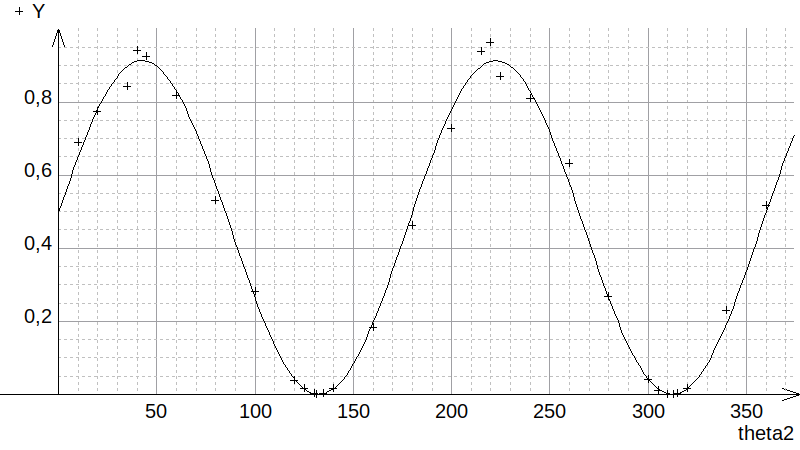
\includegraphics[scale=0.4]{pola1}
 \end{center}
\caption{Évolution de Y en fonction de l'angle de polarisation}
\end{figure}
\begin{figure}[H]
 \begin{center}
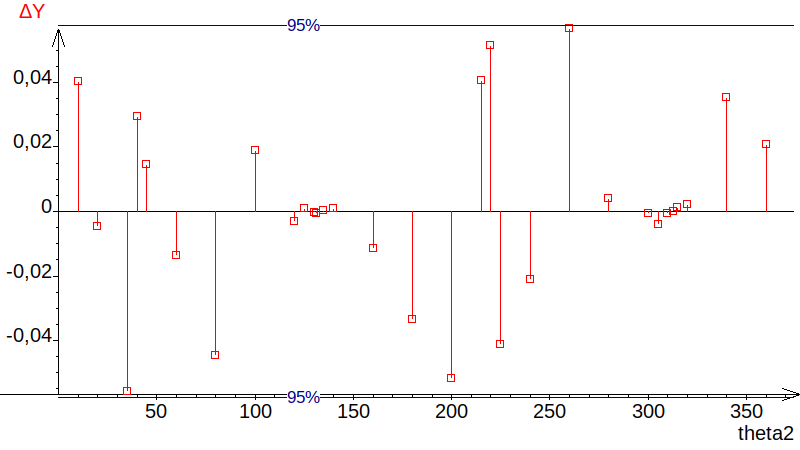
\includegraphics[scale=0.4]{pola1R}
 \end{center}
\caption{Résidus après modélisation par $\cos^2(\theta - \theta_0)$}
\end{figure}
\begin{figure}[H]
 \begin{center}
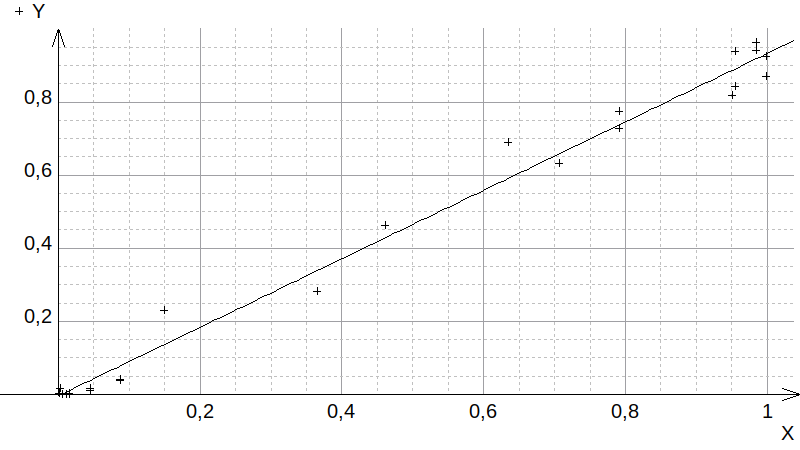
\includegraphics[scale=0.4]{pola2}
 \end{center}
\caption{Évolution de Y en fonction de $\cos^2(\theta - \theta_0)$}
\end{figure}
\subsection{Exploitation des résultats}
Théoriquement, $$Y(\theta) = \frac{P(\theta) - P_{min}}{P_{max} - P_{min}}$$. 
En remplaçant $P(\theta)$ par $P_0 \cos^2(\theta - \theta_0) + P_{offset}$ et sachant que $P_{min} = P_{offset}$ et $P_{max} = P_0 + P_{offset}$, on obtient :
$$Y(\theta) = \frac{P_0 \cos^2(\theta - \theta_0)}{P_0} = \cos^2(\theta - \theta_0)$$

On peut déduire $\theta_0$. 
Il représente l'angle d'origine (ou décalage angulaire) correspondant à la position de l'analyseur pour laquelle son axe de transmission est parfaitement aligné avec la direction de polarisation du faisceau incident, maximisant ainsi l'intensité transmise.

Regressi nous donne $\theta_0 = (44,7 \pm 1,2)^\circ$. Cependant, comme nous utilisons un polariseur Didalab, il faut rajouter ou enlever $90^\circ$ pour obtenir l'angle de transmission : $\theta_0 = (-45.3 \pm 1,2)^\circ$.

Pour montrer la linéarité, on trace $Y$ en fonction de $\cos^2(\theta - \theta_0)$. Si la polarisation est linéaire, on obtient une droite passant par l'origine de pente 1. En modélisant par une fonction affine $Y=a\times X + b$ avec Regressi, on obtient 
$a=(936 \pm21)\cdot 10^{-3} $ et $b=(-4 \pm12)\cdot 10^{-3} $ ce qui est cohérent.


% ---------------- PARTIE 2 : LAME DEMI-ONDE --------------------
\section{Action d'une lame demi-onde ($\lambda/2$)}
\subsection{Protocole}
\subsubsection{Montage expérimental}
On place la lame (5) entre deux polariseurs croisés (polariseur (2) et analyseur (3)) (extinction initiale). 
\begin{figure}[H]
 \begin{center}

\includegraphics[scale=0.7]{s2}
 \end{center}
\caption{Montage avec les polariseurs en position croisés sans lame. La lumière est bien bloquée}
\end{figure}

\begin{figure}[H]
 \begin{center}

\includegraphics[scale=0.7]{s3}
 \end{center}
\caption{Montage avec les polariseurs en position croisés avec la lame. La polarisation change et tourne de 90$^\circ$ quand la lame est tournée à 45$^\circ$ (A) et tourne à 60 $^\circ$ quand elle est tournée de 30$^\circ$.}
\end{figure}

\subsubsection{Mesures à effectuer}
\begin{enumerate}
    \item Placer 2 polariseurs en configuration croisée, le premier étant placé de façon horizontale
    \item Placer la lame sur une orientation de 0$^\circ$
    \item En faisant tourner l'analyseur, trouver les maximas et minimas.
    \item Faire tourner l'analyseur par pas de 20$^\circ$ de 0 à 360$^\circ$ et relever la puissance
    \item Refaire l'étape précédente avec une lame orientée à 30$^\circ$ puis 45$^\circ$
\end{enumerate}
\subsection{Données}
\subsubsection{Données}
\begin{table}[H]
\centering

\begin{tabular}{|c|c|c|c|c|}
\hline
\textbf{Angle $\beta$ ($^\circ$)} & \textbf{$P_0$ ($\alpha=0^\circ$)} & \textbf{$P_{30}$ ($\alpha=30^\circ$)} & \textbf{$P_{45}$ ($\alpha=45^\circ$)} & \textbf{Sans lame} \\ \hline
-90 & 3,40 & 0,73 & 0,033 & 3,71 \\ \hline
-70 & 3,26 & 1,79 & 0,29 & 3,20 \\ \hline
-50 & 2,39 & 2,98 & 1,28 & 2,36 \\ \hline
-30 & 1,22 & 3,67 & 2,56 & 1,12 \\ \hline
-10 & 0,24 & 3,32 & 3,40 & 0,20 \\ \hline
0   & 0,035 & 2,90 & 3,50 & 0,025 \\ \hline
10  & 0,057 & 2,38 & 3,62 & 0,078 \\ \hline
30  & 0,74 & 1,17 & 2,67 & 0,85 \\ \hline
50  & 1,91 & 0,21 & 1,54 & 1,87 \\ \hline
70  & 3,14 & 0,065 & 0,57 & 3,30 \\ \hline
90  & 3,51 & 0,68 & 0,028 & 3,80 \\ \hline
\end{tabular}
\caption{Mesures de la tension $U$ (V) en fonction de l'angle de l'analyseur $\beta$}
\label{tab:mesures_lame}
\end{table}
\subsubsection{Incertitudes}
La précision limitée des cadrans gradués ($\pm 0,5^\circ$) sur l'analyseur ($\Delta \beta$) et sur le support de la lame ($\Delta \alpha$) impacte directement la détermination de l'angle de rotation $\beta$. En effet, il faut prendre en compte l'incertitude des angles des 2 polariseurs en plus de celle de la lame.

L'incertitude sur la puissance lumineuse est la m\^eme qu'en partie précédente.
\subsection{Graphiques}
\begin{figure}[H]
 \begin{center}
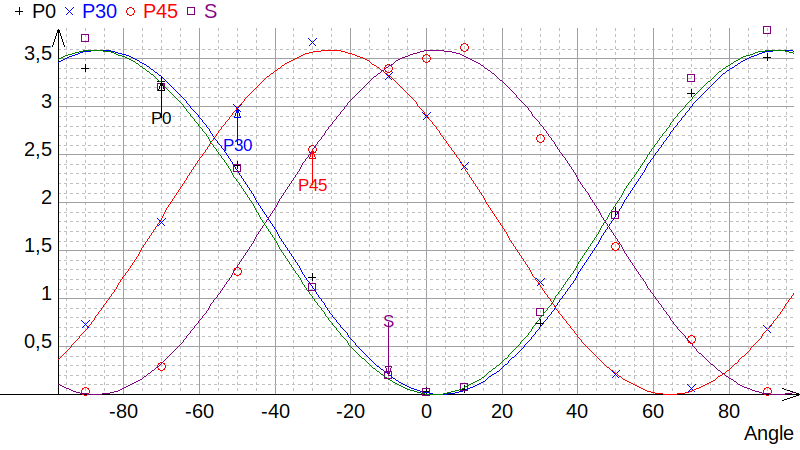
\includegraphics[scale=0.4]{pola3}
 \end{center}
\caption{Évolution de Y en fonction de l'angle de l'analyseur pour différentes valeurs d'orientation de la lame.}
\end{figure}
\subsection{Exploitation}
% L'analyse des données expérimentales permet de vérifier les propriétés de la lame demi-onde en comparant les courbes de transmission pour différentes orientations $\alpha$ de la lame par rapport à la référence sans lame.

% \begin{itemize}
%     \item \textbf{Référence et alignement ($\alpha = 0^\circ$)} : 
%     Les mesures effectuées sans lame et avec la lame orientée à $0^\circ$ sont quasi-identiques. Le maximum de tension est observé à $\beta = 90^\circ$ et le minimum à $\beta = 0^\circ$. Cela confirme que la polarisation incidente du laser est verticale et que la lame, lorsqu'elle est alignée avec l'axe de polarisation, ne modifie pas l'état de la lumière.

%     \item \textbf{Rotation de la polarisation ($\alpha = 30^\circ$ et $\alpha = 45^\circ$)} : 
%     On observe un décalage systématique des extrema de tension :
%     \begin{itemize}
%         \item Pour $\alpha = 30^\circ$, le minimum de tension se déplace vers $\beta \approx 65^\circ$. La rotation observée est proche de la valeur théorique de $2\alpha = 60^\circ$. L'écart de $5^\circ$ peut etre expliqué par les incertitudes.
%         \item Pour $\alpha = 45^\circ$, le minimum se situe exactement à $\beta = 90^\circ$ (tension résiduelle de $0,028$ V) et le maximum à $\beta = 10^\circ$. La polarisation a donc subi une rotation de $90^\circ$, ce qui est en parfait accord avec la loi $\Delta\beta = 2\alpha = 90^\circ$.
%     \end{itemize}

%     \end{itemize}

% La loi de rotation $\theta_{rot} = 2\alpha$ est vérifiée expérimentalement. La lame demi-onde permet bien de piloter la direction de polarisation du laser sans en altérer la nature rectiligne.

% Une lame demi-onde est un composant biréfringent possédant deux axes neutres orthogonaux : l'axe lent et l'axe rapide. Lorsqu'une onde polarisée rectilignement pénètre dans la lame, son champ électrique $\vec{E}$ se décompose sur ces deux axes. 

% La lame introduit un déphasage de $\Delta \phi = \pi$ (soit une demi-longueur d'onde $\lambda/2$) entre ces deux composantes. À la sortie, la superposition des composantes produit un nouveau vecteur champ électrique $\vec{E}'$ qui est le \textbf{symétrique} du vecteur incident $\vec{E}$ par rapport aux axes de la lame. 
% Géométriquement, si le champ incident fait un angle $\alpha$ avec l'axe de la lame, le champ de sortie a tourné d'un angle total :
% \begin{equation}
%     \theta_{rot} = 2\alpha
% \end{equation}

% \subsubsection*{2. Analyse de la polarisation incidente}

% D'après la série \textit{Sans lame}, nous observons un minimum d'intensité ($U \approx 0,025$~V) pour un angle de cadran $\beta_{cadran} = 0^\circ$. Comme l'axe de transmission est alors vertical ($\beta_{abs} = 90^\circ$), l'extinction prouve que le laser est polarisé \textbf{horizontalement} ($0^\circ$).



% \subsubsection*{3. Confrontation des mesures à la théorie}

% \begin{itemize}
%     \item \textbf{Cas $\alpha = 45^\circ$ :} La théorie prévoit une rotation de $2\alpha = 90^\circ$. Le champ électrique, initialement horizontal, doit devenir vertical. 
%     Expérimentalement, nous observons le maximum de tension ($U = 3,62$~V) pour $\beta_{cadran} = 10^\circ$ (soit $\beta_{abs} = 100^\circ$) et le minimum pour $\beta_{cadran} = 90^\circ$ (soit $\beta_{abs} = 180^\circ$ ou $0^\circ$). Le champ est donc bien devenu \textbf{vertical}, confirmant la rotation de $90^\circ$.
    
%     \item \textbf{Cas $\alpha = 30^\circ$ :} La rotation attendue est de $2\alpha = 60^\circ$ par rapport à l'horizontale. 
%     Sur le tableau, le maximum se déplace vers $\beta_{cadran} = -30^\circ$ (soit $\beta_{abs} = 60^\circ$). La direction du champ électrique coïncide exactement avec la prédiction théorique.
% \end{itemize}

% \subsubsection*{4. État de polarisation et résidus}

% Le fait que les minima de tension ($U_{min} < 0,1$~V) restent extrêmement faibles par rapport aux maxima ($U_{max} \approx 3,5$~V) démontre deux points essentiels :
% \begin{enumerate}
%     \item La polarisation demeure \textbf{rectiligne} après la traversée de la lame (absence d'ellipticité notable).
%     \item La lame est bien adaptée à la longueur d'onde du laser utilisé, car un déphasage différent de $\pi$ transformerait la polarisation rectiligne en polarisation elliptique, empêchant d'obtenir une extinction complète avec l'analyseur.
% \end{enumerate}

% \textbf{Conclusion :} Les mesures valident avec une grande précision le modèle de symétrie axiale de la lame demi-onde, malgré le décalage systématique dû à la conception des supports Didalab.

L'analyse repose sur la comparaison entre la référence sans lame et les séries avec lame orientée à un angle $\alpha$. Sur le matériel Didalab, l'axe de transmission réel $\beta_{abs}$ est décalé de $90^\circ$ par rapport à l'index du cadran ($\beta_{abs} = \beta_{cadran} + 90^\circ$).

\subsubsection*{1. Analyse de la polarisation incidente}
D'après la série \textit{Sans lame}, le minimum d'intensité ($U = 0,025$ V) est obtenu pour $\beta_{cadran} = 0^\circ$, soit un axe de transmission vertical ($\beta_{abs} = 90^\circ$). Cette extinction prouve que le laser est polarisé \textbf{horizontalement} ($0^\circ$).

\subsubsection*{2. Mécanisme de la lame $\lambda/2$ et confrontation théorique}
La lame demi-onde introduit un déphasage de $\pi$ entre ses axes neutres, produisant un vecteur champ électrique de sortie $\vec{E}'$ symétrique du vecteur incident par rapport à l'axe de la lame. La polarisation tourne ainsi d'un angle $\theta = 2\alpha$.

\begin{itemize}
    \item \textbf{Cas $\alpha = 45^\circ$} : La rotation théorique est de $2\alpha = 90^\circ$. La polarisation devient donc verticale. Expérimentalement, le nouveau minimum de tension se déplace bien à $\beta_{cadran} = 90^\circ$ (soit $\beta_{abs} = 180^\circ \equiv 0^\circ$, position horizontale), ce qui confirme que la lumière est devenue \textbf{verticale}.
    \item \textbf{Cas $\alpha = 30^\circ$} : La rotation théorique est de $2\alpha = 60^\circ$. La polarisation de sortie fait un angle de $60^\circ$ avec l'horizontale. On observe effectivement que le minimum de tension a "glissé" vers $\beta_{cadran} \approx 65^\circ$, ce qui correspond à une extinction pour un axe de transmission à $155^\circ$ (orthogonal à $65^\circ$). L'écart de quelques degrés s'explique par les incertitudes de positionnement des supports.
\end{itemize}



\subsubsection*{3. État de polarisation et résidus}
Les minima de tension mesurés restent extrêmement faibles ($U < 0,1$ V), ce qui démontre que :
\begin{enumerate}
    \item La polarisation demeure \textbf{rectiligne} (l'extinction est quasi-totale).
    \item La lame est parfaitement adaptée à la longueur d'onde du laser (le déphasage est bien de $\pi$).
\end{enumerate}

\textbf{Conclusion :} Les mesures valident avec précision la loi de rotation $\theta = 2\alpha$, l'écart résiduel s'expliquant par les incertitudes de positionnement des supports gradués.
% ---------------- PARTIE 3 : BREWSTER --------------------
\section{Expérience 3 : Réflexion et angle de Brewster}
\subsection{Protocole}
\begin{itemize}
    \item Plan d'incidence : Plan contenant le faisceau incident et la normale à la lame.
    \item Relation angle de mesure : $\theta_{mes} = 180 - 2\theta_i$ (selon le montage goniométrique).
    \item Polarisation : Réglée parallèlement au plan d'incidence (polarisation $p$).
\end{itemize}

\subsection{Mesures}
On cherche l'angle $\theta_B$ pour lequel la puissance réfléchie $P_r$ est minimale.
\begin{table}[H]
\centering
\begin{tabular}{|c|c|c|}
\hline
\textbf{Angle mesuré $\theta_m$ ($^\circ$)} & \textbf{Angle d'incidence $\theta_i$ ($^\circ$)} & \textbf{Puissance $P$ (u.a.)} \\ \hline
180 & 0    & 0,1400 \\ \hline
160 & 10   & 0,1400 \\ \hline
140 & 20   & 0,1300 \\ \hline
120 & 30   & 0,0990 \\ \hline
100 & 40   & 0,0610 \\ \hline
80  & 50   & 0,0220 \\ \hline
76  & 52   & 0,0170 \\ \hline
74  & 53   & 0,0133 \\ \hline
72  & 54   & 0,0098 \\ \hline
67  & 56,5 & 0,0107 \\ \hline
64  & 58   & 0,0115 \\ \hline
62  & 59   & 0,0123 \\ \hline
60  & 60   & 0,0225 \\ \hline
40  & 70   & 0,1600 \\ \hline
20  & 80   & 0,5000 \\ \hline
\end{tabular}
\caption{Mesures de la puissance réfléchie $P$ en polarisation parallèle en fonction de l'angle d'incidence $\theta_i$}
\label{tab:brewster_data}
\end{table}
\begin{table}[H]
\centering

\begin{tabular}{|c|c|c|}
\hline
\textbf{Angle mesuré $\theta_m$ ($^\circ$)} & \textbf{Angle d'incidence $\theta_i$ ($^\circ$)} & \textbf{Puissance $P$ (u.a.)} \\ \hline
160 & 10 & 0,18 \\ \hline
150 & 15 & 0,11 \\ \hline
140 & 20 & 0,12 \\ \hline
130 & 25 & 0,15 \\ \hline
120 & 30 & 0,16 \\ \hline
110 & 35 & 0,18 \\ \hline
100 & 40 & 0,20 \\ \hline
90  & 45 & 0,26 \\ \hline
80  & 50 & 0,30 \\ \hline
70  & 55 & 0,38 \\ \hline
60  & 60 & 0,47 \\ \hline
50  & 65 & 0,58 \\ \hline
40  & 70 & 0,70 \\ \hline
30  & 75 & 0,85 \\ \hline
20  & 80 & 1,02 \\ \hline
10  & 85 & 1,20 \\ \hline
\end{tabular}
\caption{Mesures de la puissance réfléchie $P$ en polarisation perpendiculaire en fonction de l'angle d'incidence $\theta_i$}
\label{tab:perpendiculaire_data}
\end{table}
\subsubsection{Incertitudes}
La précision de la détermination de l'indice de réfraction $n$ via l'angle de Brewster est limitée par plusieurs sources d'erreurs expérimentales :

\begin{itemize}
    \item \textbf{Incertitude angulaire ($\Delta \theta_i$)} : L'erreur sur le positionnement du "zéro" (incidence normale) et la résolution mécanique du goniomètre ($\pm 0,5^\circ$) impactent directement la valeur de $\theta_B$ extraite. 
    
    \item \textbf{Pureté de la polarisation ($R_\parallel$)} : Si l'axe du polariseur incident n'est pas parfaitement contenu dans le plan d'incidence, une composante perpendiculaire ($R_\perp$) subsiste. Cette imperfection explique pourquoi la puissance mesurée au minimum de Brewster ($P \approx 0,0098$) n'est pas strictement nulle.
    
    \item \textbf{Bruit de fond et linéarité du capteur} : La lumière parasite ambiante et la sensibilité de la photodiode limitent la précision des mesures, particulièrement pour les faibles puissances proches de l'extinction.
\end{itemize}

\subsection{Graphiques}
\begin{figure}[H]
    \begin{center}
        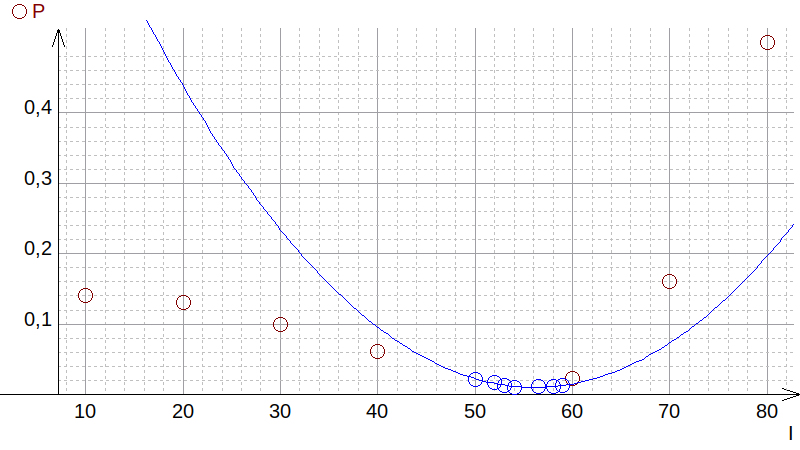
\includegraphics[scale=0.5]{bre}
    \end{center}
    \caption{Puissance réfléchie $P_r$ en fonction de l'angle d'incidence $\theta_i$ (polarisation $p$)}
\end{figure}
\subsection{Exploitation des résultats}
Au voisinage de l'angle de Brewster, on ajuste par $f(\theta_i) = A(\theta_i - \theta_B)^2 + B$. 
Regressi nous donne $\theta_b = (56,15 \pm0,34)^\circ$.

% De plus, d'après la relation de Brewster : 
% $$\tan(\theta_B) = \frac{n_{verre}}{n_{air}} \implies n_{verre} = \tan(\theta_B)$$
% On obtient ici $n_v = 1.49$, ce qui est extrèment proche de la valeur théorique attendue.
% L'incertitude est calculée via $\Delta n = (1 + \tan^2 \theta_B) \Delta \theta_B$.




\subsubsection*{Calcul de l'indice de réfraction}
D'après la loi de Brewster pour une interface air/verre ($n_{air} \approx 1$) :
\begin{equation*}
    n_v = \tan(\theta_B) = \tan(56,15^\circ) \approx 1,491
\end{equation*}

\subsubsection*{Calcul de l'incertitude}
L'incertitude $\Delta n$ est obtenue par différenciation de la relation $n = \tan \theta_B$ :
\begin{equation*}
    \dd n = \frac{\dd (\tan \theta_B)}{\dd \theta_B} \dd \theta_B = (1 + \tan^2 \theta_B) \dd \theta_B
\end{equation*}
On peut alors écrire (avec $\Delta \theta_B$ en radians) :
\begin{equation*}
    \Delta n = (1 + n^2) \cdot \left( \Delta \theta_B \cdot \frac{\pi}{180} \right)
\end{equation*}

\textbf{Application numérique :}
\begin{itemize}
    \item $\Delta n = (1 + 1,491^2) \cdot (0,34 \cdot \frac{\pi}{180}) \approx 3,22 \cdot 0,0059 \approx 0,019$
    \item Résultat : $\mathbf{n_v = 1,49 \pm 0,02}$
\end{itemize}

L'indice obtenu est en accord avec les valeurs pour le verre ($n \approx 1,50$).

\section{Conclusion}
Nous avons vérifié la loi de Malus avec un résidu faible, confirmant la polarisation rectiligne du laser. L'étude de la lame $\lambda/2$ a illustré la rotation du plan de polarisation. Enfin, la mesure de l'angle de Brewster à $\theta_B \approx 56^\circ$ permet d'identifier un indice de réfraction $n \approx 1,5$, cohérent avec celui du verre.

\end{document}